% !TeX program = pdfLaTeX
\documentclass[12pt]{article}
\usepackage{amsmath}
\usepackage{graphicx,psfrag,epsf}
\usepackage{enumerate}
\usepackage{natbib}
\usepackage{algorithm}                   
\usepackage{algpseudocode}                   
\usepackage{longtable}                   
\usepackage{booktabs}                   

\usepackage{url} % not crucial - just used below for the URL

%\pdfminorversion=4
% NOTE: To produce blinded version, replace "0" with "1" below.
\newcommand{\blind}{0}

% DON'T change margins - should be 1 inch all around.
\addtolength{\oddsidemargin}{-.5in}%
\addtolength{\evensidemargin}{-.5in}%
\addtolength{\textwidth}{1in}%
\addtolength{\textheight}{1.3in}%
\addtolength{\topmargin}{-.8in}%

\begin{document}

\def\spacingset#1{\renewcommand{\baselinestretch}%
{#1}\small\normalsize} \spacingset{1}


%%%%%%%%%%%%%%%%%%%%%%%%%%%%%%%%%%%%%%%%%%%%%%%%%%%%%%%%%%%%%%%%%%%%%%%%%%%%%%

\if0\blind
{
  \title{\bf Fundamental Kernel Density Estimation for Computation}

  \author{
        Michael Liou \thanks{All code is available at www.github.com/lioumens/stat771\_final} \\
    Department of Statistics, University of Wisconsin, Madison\\
      }
  \maketitle
} \fi

\if1\blind
{
  \bigskip
  \bigskip
  \bigskip
  \begin{center}
    {\LARGE\bf Fundamental Kernel Density Estimation for Computation}
  \end{center}
  \medskip
} \fi

\bigskip
\begin{abstract}
We cover fundamental principles of the Kernel Density Estimate (KDE) in
a computational setting. Influence of kernel choice and bandwidth tuning
on the density estimates are illustrated. Asymptotic bounds and decision
theoretic frameworks are presented for the KDE. Computational complexity
and efficiency of the Fast Fourier Transform (FFT) procedure in KDE
calculation are shown, and bandwidth choices are also shown to nearly
attain the asymptotic lower bound computationally. Multivariate
extensions of the univariate first principles are briefly mentioned.
\end{abstract}

\noindent%
{\it Keywords:} nonparametric, statistics, fast fourier transform, curse of dimensionality
\vfill

\newpage
\spacingset{1.45} % DON'T change the spacing!

\newcommand{\expect}[1]{\mathbf{E}\left[ #1 \right]}
\newcommand{\variance}[1]{\mathrm{Var}\left( #1 \right)}
\newcommand{\covariance}[1]{\mathrm{Cov}\left( #1 \right)}
\newcommand{\bigo}[1]{\mathcal{O}\left( #1 \right)}

\def\tightlist{}

\section{Introduction}\label{introduction}

Density estimation is a useful, nonparametric way to estimate the
underlying probability density function. This is common in any scenario
in which we are trying to determine a pattern of the underlying random
process from an observed dataset. Density estimation can provide insight
to the pattern of the underlying distribution, especially when the
underlying distribution is complicated. Here, we explore some of the
fundamental computational results that have shaped the univariate
density estimation. We then extend some of these principles into a
multidimensional setting and look at how current research areas have
addressed sparsity issues and parameter tuning in higher dimensions. We
illustrate these results with a mix of mature code bases and self-coded
crude approximations.

\section{Theoretical Background}\label{theoretical-background}

\subsection{Estimators}\label{estimators}

The kernel density estimator with bandwidth \(h > 0\) and kernel \(K\)
is defined as

\[
\begin{aligned}
\hat{f_n}(x) = \frac{1}{n} \sum_{i=1}^{n} \frac{1}{h} K\left(\frac{x-X_i}{h}\right)
\end{aligned}
\]

There are two parameters to specify for this estimator, the kernel \(K\)
and the bandwidth \(h\). It is well known from theory and practice that
the kernel does not have a significant on the final density estimate. On
the other hand, the bandwidth will have a large effect on the overall
fit of the estimate. The bandwidth determines the scaling parameter of
the kernel. Visually, the bandwidth determines how ``squiggly'' the
estimate looks. The KDE estimate at one particular point is the sum of
the Gaussian kernel at every point of evaluation.

\begin{figure}[h]
\label{fig:bandwidth}
\caption{Comparison of different bandwidths}
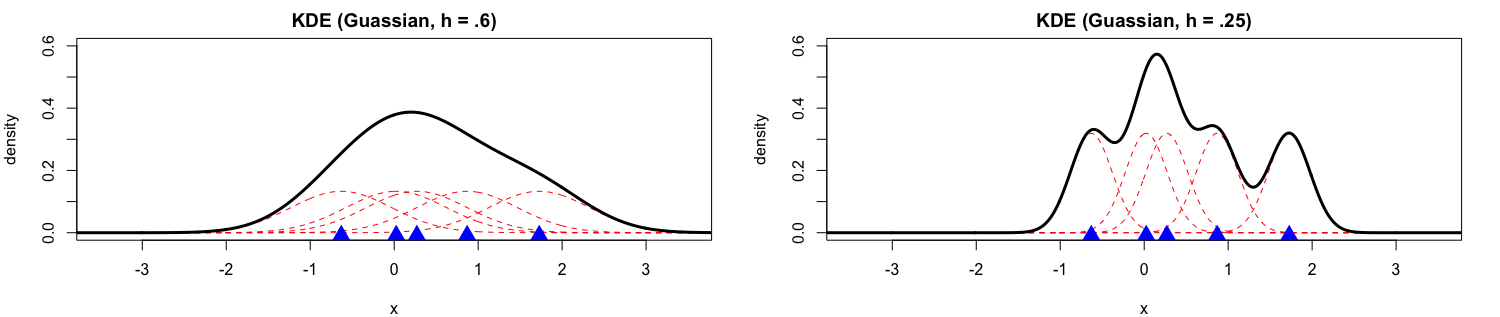
\includegraphics[scale=.31]{bandwidth_fig}
\end{figure}

\begin{figure}[h]
\caption{Comparison of different kernels}
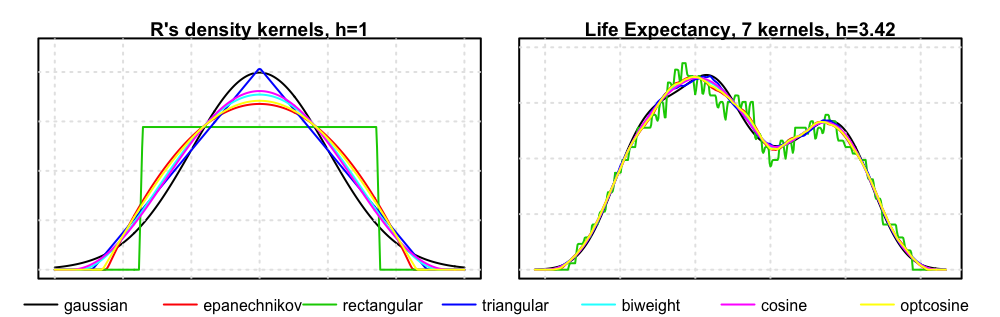
\includegraphics[scale=.4]{fig2}
\centering
\end{figure}

The difficulty with kernel density estimation is the varying regions of
high density and low density sample regions, in which low bandwidth more
appropriate for low density regions and high bandwidth is more
appropriate for high density regions. Thus, many other estimators that
build off of this basic idea have been proposed
\citep{silverman2018density, MACK19791, silverman1982estimation, mack1979multivariate}.

\begin{longtable}[]{@{}lll@{}}
\caption{Non-Exhaustive List of Density Estimators}\tabularnewline
\toprule
\begin{minipage}[b]{0.20\columnwidth}\raggedright\strut
Estimator\strut
\end{minipage} & \begin{minipage}[b]{0.32\columnwidth}\raggedright\strut
Formula\strut
\end{minipage} & \begin{minipage}[b]{0.38\columnwidth}\raggedright\strut
Defined Terms\strut
\end{minipage}\tabularnewline
\midrule
\endfirsthead
\toprule
\begin{minipage}[b]{0.20\columnwidth}\raggedright\strut
Estimator\strut
\end{minipage} & \begin{minipage}[b]{0.32\columnwidth}\raggedright\strut
Formula\strut
\end{minipage} & \begin{minipage}[b]{0.38\columnwidth}\raggedright\strut
Defined Terms\strut
\end{minipage}\tabularnewline
\midrule
\endhead
\begin{minipage}[t]{0.20\columnwidth}\raggedright\strut
Adaptive Smooth (Location)\strut
\end{minipage} & \begin{minipage}[t]{0.32\columnwidth}\raggedright\strut
\(\frac{1}{nh(x)} \sum^{n}_{i=1}{K \left( \frac{x-X_i}{h(x)}\right)}\)\strut
\end{minipage} & \begin{minipage}[t]{0.38\columnwidth}\raggedright\strut
\(h(x)\) is a function of the location \(x\)\strut
\end{minipage}\tabularnewline
\begin{minipage}[t]{0.20\columnwidth}\raggedright\strut
Adaptive Smooth (Sample)\strut
\end{minipage} & \begin{minipage}[t]{0.32\columnwidth}\raggedright\strut
\(\frac{1}{n} \sum^{n}_{i=1}{\frac{1}{h_i}K \left( \frac{x-X_i}{h_i}\right)}\)\strut
\end{minipage} & \begin{minipage}[t]{0.38\columnwidth}\raggedright\strut
\(h_i\) is a function of the \(i\)th sample point\strut
\end{minipage}\tabularnewline
\begin{minipage}[t]{0.20\columnwidth}\raggedright\strut
Nearest Neighbor\strut
\end{minipage} & \begin{minipage}[t]{0.32\columnwidth}\raggedright\strut
\(\frac{1}{nd_k(x)} \sum^{n}_{i=1}{K \left( \frac{x-X_i}{d_k(x)}\right)}\)\strut
\end{minipage} & \begin{minipage}[t]{0.38\columnwidth}\raggedright\strut
\(d_k(x)\) is the Euclidean distance between \(x\) and the increasing
\(k\)th nearest neighbor sequence\strut
\end{minipage}\tabularnewline
\begin{minipage}[t]{0.20\columnwidth}\raggedright\strut
Orthogonal Series\strut
\end{minipage} & \begin{minipage}[t]{0.32\columnwidth}\raggedright\strut
\(\sum^{n}_{i=1}\theta_i\phi_i(x)\)\strut
\end{minipage} & \begin{minipage}[t]{0.38\columnwidth}\raggedright\strut
\(\phi_i\) is an orthogonal basis,
\(\theta = \expect{ \frac{1}{n} \sum_i\phi_i(x)}\)\strut
\end{minipage}\tabularnewline
\begin{minipage}[t]{0.20\columnwidth}\raggedright\strut
Max Penalized Likelihood\strut
\end{minipage} & \begin{minipage}[t]{0.32\columnwidth}\raggedright\strut
\(\arg \max_{f} \frac{1}{n} \sum^{n}_{i=1}\log f(X_i)- \frac{1}{2}\lambda\left[\log f, \log f\right]\)\strut
\end{minipage} & \begin{minipage}[t]{0.38\columnwidth}\raggedright\strut
\(\left[f,f\right] = \int D(f)D(f)\), \(D(f)\) is linear differential
operator\strut
\end{minipage}\tabularnewline
\bottomrule
\end{longtable}

\pagebreak

\subsection{Decision theory}\label{decision-theory}

In order to evaluate an estimator in a decision theoretic framework, a
commonly defined loss function is the Mean Integrated Squared Error
(MISE), which averages the estimator's performance over all samples that
could be observed. We can show that, under some regularity conditions,
there is a bias-variance trade-off with the MISE.

\begin{equation} \label{mise}
\begin{split}
\mathrm{MISE}(\hat{f}) &= \expect{\int_{-\infty}^{\infty}(\hat{f}(x) - f(x))^2 \, dx} \\
&= \int_{-\infty}^{\infty}\expect{(\hat{f}(x) - f(x))^2} \, dx \\
&= \int_{-\infty}^{\infty} \variance{\hat{f}(x)} + \left(\mathrm{bias}(\hat{f}(x))\right)^2 \, dx
\end{split}
\end{equation}

To calculate the bias term for the kernel density estimator, we
substitute a Taylor expansion and integrate.

\[
\begin{aligned}
\expect{\hat{f}(x)} &= f(x) + \frac{1}{2}h^2\sigma^2_Kf''(x) + o(h^2) \\
\left[\expect{\hat{f}(x)} - f(x)\right]^2 &= \frac{1}{4}h^4\sigma^4_K\left(f''(x)\right)^2 + o(h^4) \\
\int \left[\expect{\hat{f}(x)} - f(x)\right]^2 \, dx &= \frac{1}{4}h^4\sigma^4_K\left(\int f''(x)^2 \, dx\right) + o(h^4) 
\end{aligned}
\] To calculate the variance term, we do a Taylor expansion about \(x\),
and change of variable \(t = \frac{x-X_i}{h}\).

\[
\begin{aligned}
\variance{\hat{f}(x)} &= \frac{1}{nh}\int K(t)^2f(x-ht)\, dt - \frac{1}{n}\left[\expect{ \frac{1}{h} K\left( \frac{x-X_i}{h}\right)}\right]^2 \\
&= \frac{1}{nh}\int K(t)^2[f(x) + o(1)] \, dt - \frac{1}{n}\left[f(x) + o(1)\right]^2\\
&= \frac{1}{nh}f(x) \left(\int K(t)^2\, dt\right) + o\left( \frac{1}{nh}\right) \\
\int \variance{\hat{f}(x)} \, dx &= \frac{1}{nh}\left(\int K(t)^2\, dt\right) + o\left( \frac{1}{nh}\right)
\end{aligned}
\] Hence, if we put these together back into MISE, we can evaluate our
density estimate as a function of the bandwidth parameter and the data.
The terms without the order approximation is know as the Asymptotic MISE
(AMISE) \citep{wasserman2006all}.

\[
\begin{aligned}
MISE(h) &= \frac{1}{nh}\left(\int K(t)^2\, dt\right) + \frac{1}{4}h^4\sigma^4_K\left(\int f''(x)^2 \, dx\right) + o \left( \frac{1}{nh} + h^4\right)
\end{aligned}
\] We often estimate this term with cross-validation, with an estimator
off by a true constant term.

\begin{equation}
\label{est_risk}
\hat J(h) = \int \left(\hat{f_n}(x)\right)^2 \, dx - \frac{2}{n} \sum^{n}_{i=1}{ \hat{f}_{(-i)}(X_i)}
\end{equation}

\subsection{Bandwidth Estimation}\label{bandwidth-estimation}

Since good bandwidth choice has shown to be highly influential on the
quality of the density estimate, many rules have been developed to
choose a good bandwidth. Some of the more common methods are shown
briefly below

\begin{longtable}[]{@{}ll@{}}
\toprule
\begin{minipage}[b]{0.37\columnwidth}\raggedright\strut
Name of Rule\strut
\end{minipage} & \begin{minipage}[b]{0.57\columnwidth}\raggedright\strut
Estimation Procedure\strut
\end{minipage}\tabularnewline
\midrule
\endhead
\begin{minipage}[t]{0.37\columnwidth}\raggedright\strut
Silverman's Rule of Thumb\strut
\end{minipage} & \begin{minipage}[t]{0.57\columnwidth}\raggedright\strut
\(h_n = \left( \frac{4 \hat{\sigma}^5}{3n}\right)^{1/5}\) where
\(\hat\sigma = \min\left(s, \frac{IQR}{1.34}\right)\)\strut
\end{minipage}\tabularnewline
\begin{minipage}[t]{0.37\columnwidth}\raggedright\strut
Sheather-Jones\strut
\end{minipage} & \begin{minipage}[t]{0.57\columnwidth}\raggedright\strut
See \citep{SJ}\strut
\end{minipage}\tabularnewline
\begin{minipage}[t]{0.37\columnwidth}\raggedright\strut
Cross-Validation\strut
\end{minipage} & \begin{minipage}[t]{0.57\columnwidth}\raggedright\strut
See \citep{scott_terrell}\strut
\end{minipage}\tabularnewline
\bottomrule
\end{longtable}

\begin{figure}[h]
\label{fig:bw_selection}
\caption{Comparison of Bandwidth Selection Rules}
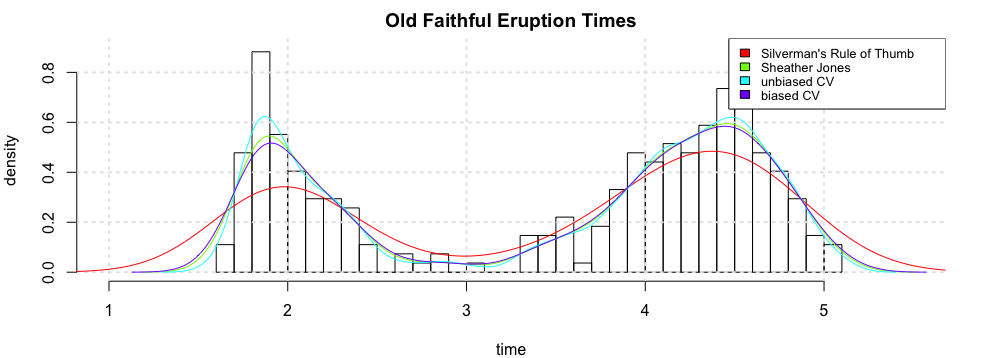
\includegraphics[scale=.5]{bw_selection}
\centering
\end{figure}

\subsection{Curse of Dimensionality}\label{curse-of-dimensionality}

Density estimation in practice is generally used with lower dimensional
data. Consider a sample
\(\mathbf{x_1},\mathbf{x_2}, \ldots, \mathbf{x_n}\) from a
\(d\)-dimensional density function \(f\). As the sample space increases
in dimension, the pairwise distance between each of the points
increases, and our space will be increasingly sparse, making it more
difficult to estimate the underlying density function. We would thus
require an exponentially increasing amount of data corresponding to the
dimension to achieve a similar MSE lower bound. This is known as the
\emph{curse of dimensionality} \citep{scott2015multivariate}. We focus
on the kernel density estimator. In higher dimensions, our general
kernel density estimator is defined by

\[
\begin{aligned}
\hat{f}_n(\mathbf{x}) = \frac{1}{n} \sum^{n}_{i=1}{|\mathbf{H}|^{-1/2}K\left(\mathbf{H}^{-1/2}(\mathbf{x} - \mathbf{X_i})\right)}
\end{aligned}
\]

For higher dimensions, it has been shown that the optimal MISE for an
estimator runs on the order of \(\bigo{n^{-4/(d+4)}}\). Based on this
lower bound for MSE, we see that as \(n\rightarrow \infty\) our
estimator \(\hat{f}(x)\) converges in probability to \(f(x)\). The
bandwidth selection also becomes more difficult because instead of a
single parameter, we must now estimate a matrix of bandwidths.

\section{Computation}\label{computation}

\subsection{Using the FFT}\label{using-the-fft}

In situations the density estimate needs to be calculated on a grid of
points, such as plotting, calculating the kernel density estimator
directly is inefficient, requiring \(\bigo{n^22^g}\) time to run on a
dataset with \(n\) data points and \(g\) grid points. If we note that
the kernel density estimate is simply a convolution of the empirical
density function \(g(x) = \frac{1}{n} \sum_{i=1}^{n}\delta(x-x_i)\)
(where \(\delta\) is the generalized Dirac delta function) and the
symmetric kernel \(K_h(x)\) with bandwidth parameter \(h\), we can
utilize the Fast Fourier Transform to reduce the computational
complexity to \(\bigo{ng\log n}\)
\citep{wand1994fast, lohne2017computational}. This calculation, due to
rounding and underflow, the estimate of the density may lead to small
negative values in some cases. We can simply smooth these estimates by
setting them to zeros \citep{silverman1982algorithm}. This is the method
(slightly simplified) used by the function \texttt{density()} in
\texttt{R}. The number of grid points we discretize the space will also
have a significant effect on the algorithm speed. In particular, the
direct calculation will grow exponentially with the grid we discretize
over.

\begin{algorithm}[H]
\caption{Univariate KDE with Fast Fourier Transform}
\begin{algorithmic}
\Function{KDE\_FFT}{$X$, Bandwidth}
  \State mesh $\gets [\min X - \mathrm{sd}(X), \max X + \mathrm{sd}(X)]$
  \State meshcount $\gets \mathrm{hist}(X, \mathrm{mesh})$
  \State meshkernel $\gets \mathrm{dKern}(\mathrm{mesh})$ \Comment{density values of kernel over mesh}
  \State density $\gets \mathrm{FFT}^{-1}(\mathrm{FFT}(\mathrm{meshcount}) * \mathrm{FFT}(\mathrm{meshkernel}))$
  \State density $\gets$ SmoothZeros(density)
  \State \Return density
\EndFunction
\end{algorithmic}
\end{algorithm}

\begin{figure}[h]
\caption{Old Faithful Data (N=272)}
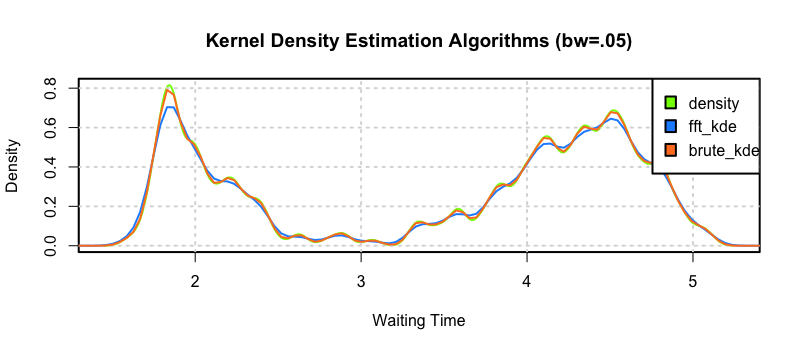
\includegraphics[scale=.5]{density_comparison}
\centering
\label{fig:plot1}
\end{figure}

The routines \texttt{brute\_kde()} and \texttt{fft\_kde()} were coded
myself from scratch, and we compare computational speeds to
\texttt{density()} provided by \texttt{R} in the univariate case on the
eruption times of the Old Faithful Geyser Data in Yellowstone National
Park \citep{azzalini1990look}. For comparability, we calculate the
discretization over a grid of \(512\) points which is default for the
\texttt{density()} function. From Figure \ref{fig:plot1} we can see that
all the algorithms seem to match up fairly well on our Old Faithful
Eruption data. We can attribute the slight deviations to rounding errors
and having used a different discrete grid. From Table 3 we see that
there is over \(1000x\) speed-up from using a brute force approach to
using the FFT. Our hand coded algorithm is also slightly faster than the
standard \texttt{density()} function. This is likely because we do not
do error checking or argument processing in our algorithms, such as
weights or kernel changing.

\begin{longtable}[]{@{}llll@{}}
\caption{Computational Time comparison (avg of 10 runs)}\tabularnewline
\toprule
Algorithm & \texttt{brute\_kde} & \texttt{fft\_kde} & \texttt{density}
from R\tabularnewline
\midrule
\endfirsthead
\toprule
Algorithm & \texttt{brute\_kde} & \texttt{fft\_kde} & \texttt{density}
from R\tabularnewline
\midrule
\endhead
Time(s) & 0.3667 & 0.000464 & 0.00073\tabularnewline
\bottomrule
\end{longtable}

\begin{figure}[h]
\label{fig:gs}
\caption{Comparison of Algorithms dependency on Gridsize}
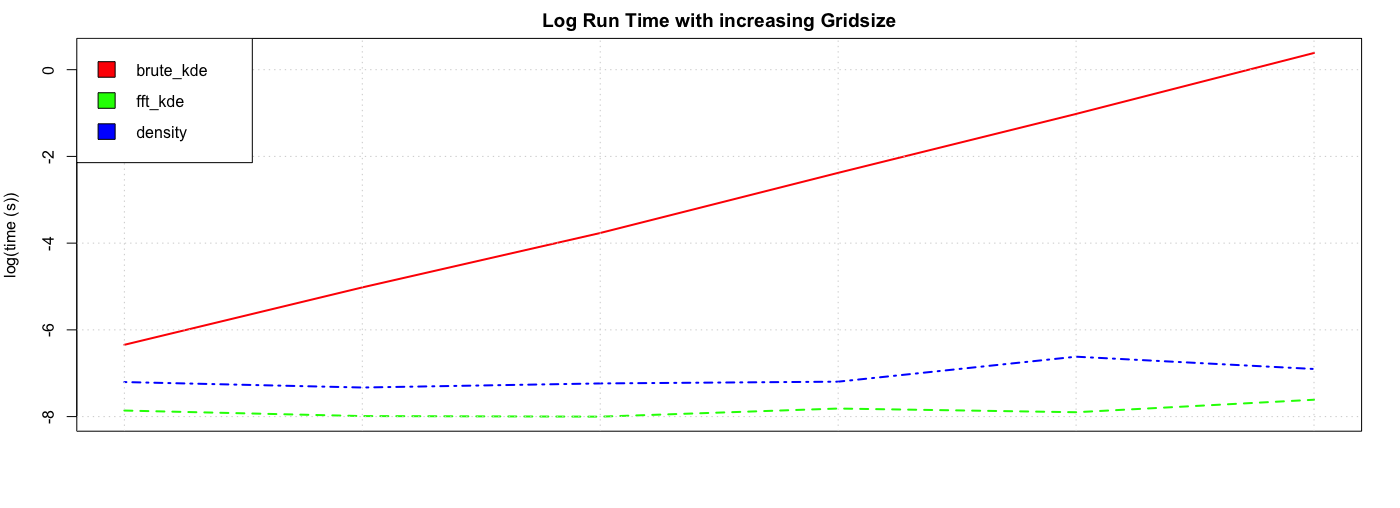
\includegraphics[scale=.3]{gridsize_time}
\centering
\end{figure}

\subsection{Accuracy with Data}\label{accuracy-with-data}

In the above theoretical work, we saw that in the univariate case, the
best estimator with optimal bandwidth selection would have a convergence
rate of \(\bigo{n^{-4/5}}\) as a function of the number of data points
\(n\). We illustrate the result by calculating the cross-validated risk
estimator as shown in Eq. \ref{est_risk} with a near-optimal bandwidth
selector, Silverman's Rule of Thumb.

\begin{figure}[h]
\centering
\label{fig:kde_data}
\caption{The KDE estimator with Silverman's Rule of Thumb converges closer and closer to the ``true" distribution with more data. Faded densities are estimates with less data.}
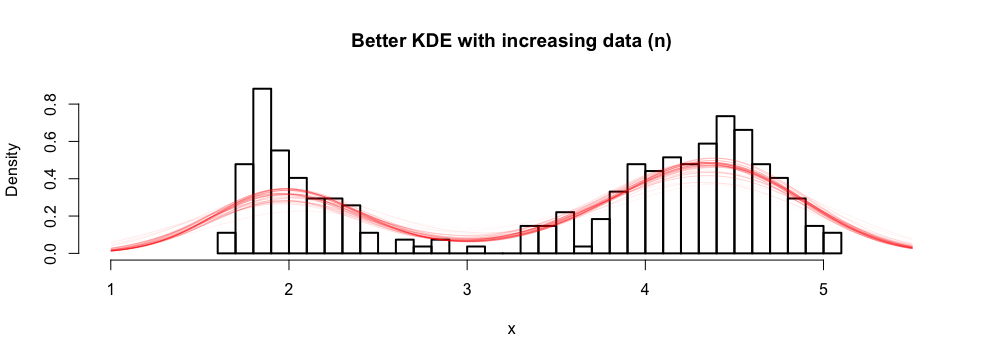
\includegraphics[scale=.5]{kde_data}
\end{figure}

\begin{figure}[h]
\centering
\label{fig:lb}
\caption{Estimated risk of estimator with increasing data nears the theoretical lower bound of $n^{-4/5}$}
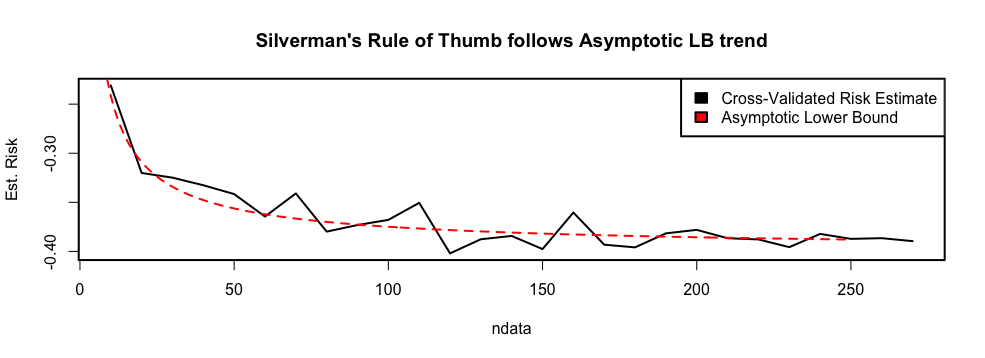
\includegraphics[scale=.5]{lb_silverman}
\end{figure}

\subsection{Higher Dimensions}\label{higher-dimensions}

Again, we would like to use the FFT in higher dimensions because of the
massive computational speedup for calculating the KDE. Here we present a
two dimensional example based on a UNICEF dataset on life expectancy and
child mortality. The problem of using a definitive FFT-based algorithm
for unconstrained bandwidth matrices is an open question, though some
significant progress was made recently \citep{fft_unconstrained}. The
technical details are omitted, but the main result is an observation
that the generalization presented in \citep{wand1994kernel}, has two
orderings, the \emph{zero-padding} and \emph{wrap-arround ordering}. The
wrap-around ordering will only support kernels that are oriented with
the axes, and thus, reshaping the FFT input matrix to use only zero
padded procedures will remove some symmetry aliasing. This order was
causing some irregularity in the density estimate as shown in Figure
\ref{fig:unconstrainedH}. They also suggest a scaling parameter of the
mesh size based on the largest eigenvalue of the bandwidth matrix
\(\mathbf{H}\). This is an interesting result, but doesn't guarantee
that weaknesses will not be found with the zero-padded ordered matrix.
This result has already been integrated into the package \texttt{ks} in
\texttt{R}.

\begin{figure}[h]
\centering
\caption{Reproduction of Figure 1 of (Gramacki \& Gramacki 2017) showing weakness of KernSmooth FFT implementation. Note (a) is different from (b) and (c)}
\label{fig:unconstrainedH}
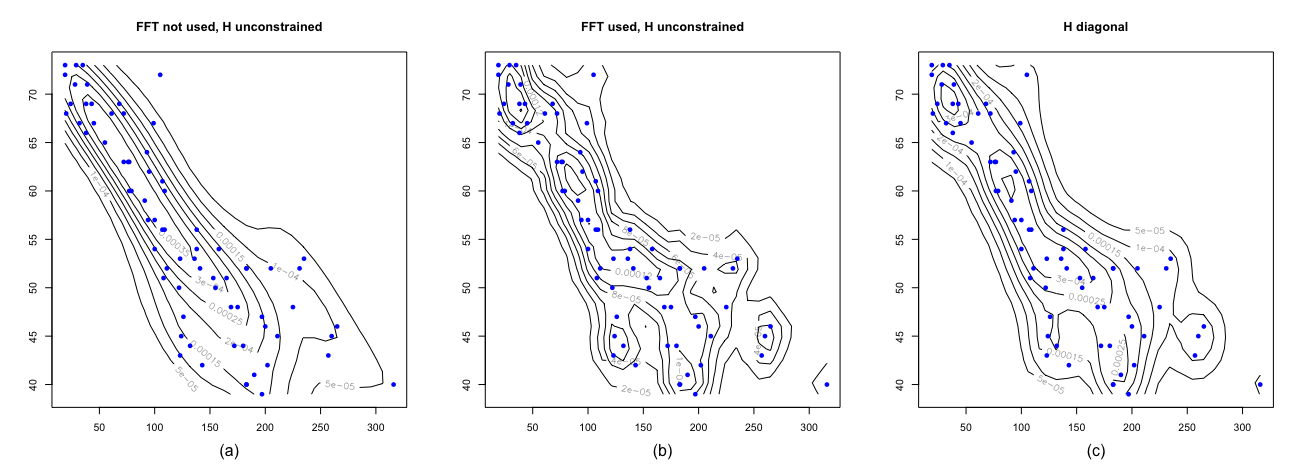
\includegraphics[scale=.33]{fig1_unconstrained}
\end{figure}

\section{Conclusions}\label{conclusions}

Density estimation has seen many useful applications for understanding
of underlying data structure or as a first step in downstream analysis.
We've shown some asymptotic results that have led to a wide array of
other estimators, in particular the kernel density estimate. The quality
of the KDE is highly subject to bandwidth changes, but less so to the
kernel choice. The fundamental computational results in one dimension of
using the FFT was explored, and we can see at least a 1000-fold increase
in computational speed depending on the chosen gridsize. We note the
work of extending these results to the multivariate case has matured
significantly since the 1990s, which has reduced the computational
complexity and increased the accuracy to the point they have been
integrated into common software packages \citep{chen2017tutorial}. In
future years, we are excited to see maturity in other density estimation
techniques such as orthogonal series estimators, splines, or tree-based
density estimation.

\bibliographystyle{agsm}
\bibliography{bibliography.bib}

\end{document}
